\begin{table*}[h]\footnotesize
    \centering
    \caption{Contents and declaration methods of XML elements}
    \label{tab:xml-elements}
    
    \rowcolors{3}{white}{lightgray}    

    \begin{tabu} to \textwidth { l | c c c | X }
        \hline
            XML element             &   Text    &   Elements    &   Attributes      &   Declaration method     \\
                                    % &   Text    &   Elements    &   Attributes      &                    \\
        \hline
            Simple                  &   Yes     &   No          &   No              &   \texttt{xs:simpleType}                       \\
            Complex empty           &   No      &   No          &   Yes             &   \texttt{xs:complexType} + [\texttt{xs:complexContent}] + attributes \\
            Complex text-only       &   Yes     &   No          &   Yes             &   \texttt{xs:complexType} + \texttt{xs:simpleContent}  + attributes \\
            Complex element-only    &   No      &   Yes         &   Yes             &   \texttt{xs:complexType} + [\texttt{xs:complexContent}] + elements + attributes \\
            Complex mixed           &   Yes     &   Yes         &   Yes             &   \texttt{xs:complexType} + [\texttt{xs:complexContent}] + \newline \texttt{mixed} flag + elements + attributes \\
        \hline
    \end{tabu}
\end{table*}

\subsubsection{XSD-based data models}\label{sec:xsd-based-data-models}

\paragraphx{\\XML elements and XSD types}

Similarly to EXPRESS-based data models, a XSD-based data model is described using one or more interrelated XSD schemas.
Each schema is a kept in a separate document and then the document can be imported by other XSD schemas or XML documents.
For instance, the CityGML data model consists of many XSD schemas, which address specific subdomains such as bridge, building, city furniture, land use, tunnel, etc.
These schemas import other base XSD schemas, such as GML and CityGMLBase.



An XML schema contains declarations of XML elements, their attributes, and related types.
There are two kinds of XML elements: simple and complex.
\emph{Simple elements} can only have text, whereas \emph{complex elements} can contain text, elements, and attributes.
Complex elements also have four subkinds: empty, text-only, elements-only, and mixed.
\autoref{tab:xml-elements} describes possible contents and declaration methods of XML elements to facilitate their recognition.






% \begin{table}\footnotesize
%     \centering
%     \caption{Kinds of XML elements}
%     \label{tab:xml-elements}
    
%     \rowcolors{2}{white}{lightgray}    
    
%     \begin{tabu} to \columnwidth { X c c c }
%         \hline
%             XML element             &   Text    &   Elements    &   Attributes  \\
%         \hline
%             Simple                  &   Yes     &   No          &   No          \\
%             Complex Empty           &   No      &   No          &   Yes         \\
%             Complex Text-only       &   Yes     &   No          &   Yes         \\
%             Complex Element-only    &   No      &   Yes         &   Yes         \\
%             Complex Mixed           &   Yes     &   Yes         &   Yes         \\
%         \hline
%     \end{tabu}
% \end{table}


As can be seen in \autoref{tab:xml-elements}, there are two XSD types.
\emph{Simple types} (\texttt{xs:simpleType}) are used for declaring simple elements or attributes, which only have text content.
\emph{Complex types} (\texttt{xs:complexType}) are applied only for complex elements.
Each type has a base type.
The top base type for simple types is \texttt{xs:anySimpleType}, and the top base type for all types is \texttt{xs:anyType}.

XSD allows to specify a simple type as a list (\texttt{xs:list}) of another simple type, or as a union (\texttt{xs:union}) of other simple types.
Moreover, XSD provides multiple restrictions (\texttt{xs:restriction}) for simple types:
\begin{itemize}
    \item \texttt{enumeration} defines a list of acceptable values.
    \item \texttt{length}, \texttt{min\-Length}, and \texttt{max\-Length} define a number of string characters or list items.
    \item \texttt{min\-Inclu\-sive}, \texttt{max\-Inclu\-sive}, \texttt{min\-Exclu\-sive}, and \texttt{max\-Exclu\-sive} define lower and upper bounds for numeric values.
    \item \texttt{pattern} defines a character pattern for string values.
    \item \texttt{totalDigits} and \texttt{fractionDigits} define numbers of digits in total and after the decimal point allowed in a number.
\end{itemize}



Complex types can include the following declarations: element (\texttt{xs:element}), element group (\texttt{xs:group}), attribute (\texttt{xs:attribute}), attribute group (\texttt{xs:attri\-bute\-Group}), \emph{any}-element (\texttt{xs:any}), and \emph{any}-attribute (\texttt{xs:anyAttribute}).
Any-elements and any-attributes are elements and attributes undefined by the schema.
Elements in a complex type or a element group must be defined with exact one of \emph{order indicators}:
(i) \texttt{sequence} allows child elements to occur in any order;
(ii) \texttt{all} allows child elements to occur in the order as defined;
and (iii) \texttt{choice} allows only one of the child elements to occur.
Regardless of which order indicator is used, elements can be specified with \texttt{min\-Occurs}, \texttt{max\-Occurs} and \texttt{nillable} attributes.
Unlike elements of a complex type, attributes may occur in an element not more than once.
However, attributes can be declared as \texttt{optional} or \texttt{required}.


All elements and attributes have their own names, which are unique inside their parent element.
Whereas, XSD types can be anonymous when they are wrapped inside their only owner (element or parent type).
Besides, all elements, attributes, and types can have annotations formatted with \texttt{xs:annotation} and \texttt{xs:documentation}.

One element can replace another by declaring \texttt{substitutionGroup} attribute.
Elements which can be replaced are usually defined with the \texttt{abstract} flag, but not always.
Complex types also can be abstract.
Complex elements can only have non-abstract complex types.


% Unique keys?



\bigskip\paragraphx{XSD-based building data formats}


Although XSD allows describing almost any data model, building data formats based on entity-based conceptual models utilise only certain element structures and types.
A few common practices of representing entity-based conceptual models as XSD schemas are described in \autoref{tab:entity-models-to-xsd}.
It can also facilitate the understanding of how entity models could be converted back from these XSD schemas.
The list of XSD-based data formats taken for the analysis are the followings: IFC-XML (ifcXML), COBieLite, CityGML, bsDD, and LandXML.

\begin{table}[h]\footnotesize
    \centering
    \caption{Contents and declaration methods of XML elements}
    \label{tab:xml-elements}
    
    \rowcolors{3}{white}{lightgray}    
    \begin{threeparttable}
        \begin{tabu} to \columnwidth { p{1.8cm} X[l] }
            \hline
                Data model item  &   XML construct         \\
            \hline
                Entity            &   Complex element
                      \\
                Entity attribute            &   Attribute or complex element
                      \\
                Entity type            &   
                    \texttt{xs:complexType} + [\texttt{xs:complexContent}]\tnotex{tnote:mixed-flag} \newline
                    + \texttt{xs:sequence}\tnotex{tnote:choice-instead-sequence} + elements + attributes  \\
                Select type            &   
                    \texttt{xs:complexType} + [\texttt{xs:complexContent}] \newline
                    + \texttt{xs:choice} + elements  \\
                Enumeration type &   
                    \texttt{xs:simpleType}  +  \texttt{xs:restriction} + \texttt{xs:enumeration} \\
                Defined type \newline based on \newline a primitive type &   
                    \texttt{xs:simpleType}  \\
                % Defined type \newline based on a primitive type &   
                    % \texttt{xs:simpleType}  \\
                Primitive type &
                    Not declared \\
            \hline
        \end{tabu}
        \begin{tablenotes}
          \item\label{tnote:mixed-flag} \texttt{mixed} flag can be is used, but rarely.
          \item\label{tnote:choice-instead-sequence} If there is only one element, \texttt{xs:choice} can be used instead.
        \end{tablenotes}
    \end{threeparttable}
\end{table}





Assume that we have an entity-based conceptual model.
Then its entity types can be mapped into either complex empty, or complex element-only, or complex mixed elements.
Entity attributes are represented as XML attributes, if their types can be mapped into XML simple types.
Otherwise, entity attributes are represented as XML elements wrapped in the parent complex element.
Wrapped elements of Complex Element-only or Complex Mixed elements are usually specified with order indicator \texttt{xs:sequence}.
However, if there is only one internal element, order indicator \texttt{xs:choice} also can be used.
In contrast, order indicator \texttt{xs:any} must be avoided.
Complex Mixed elements are used very rarely and mainly for addresses types (see \autoref{lst:xsd-entity-type-mixed-element}).

\begin{lstlisting}[caption={a},label=lst:xsd-entity-type-mixed-element]
<xs:element name="PostBoxNumberPrefix" minOccurs="0">
  <xs:annotation>
    <xs:documentation>Specification of the prefix of the post box number. eg. A in POBox:A-123</xs:documentation>
  </xs:annotation>
  <xs:complexType mixed="true">
    <xs:attribute name="NumberPrefixSeparator">
      <xs:annotation>
        <xs:documentation>A-12 where 12 is number and A is prefix and "-" is the separator</xs:documentation>
      </xs:annotation>
    </xs:attribute>
    <xs:attributeGroup ref="grPostal"/>
    <xs:anyAttribute namespace="##other"/>
  </xs:complexType>
</xs:element>
\begin{lstlisting}



\begin{lstlisting}[caption={a},label=lst:xsd-entity-type]
<xs:element name="IfcAppliedValue" type="ifc:IfcAppliedValue" substitutionGroup="ifc:Entity" nillable="true"/>
  <xs:complexType name="IfcAppliedValue">
    <xs:complexContent>
      <xs:extension base="ifc:Entity">
        <xs:sequence>
          <xs:element name="AppliedValue" nillable="true" minOccurs="0">
            <xs:complexType>
              <xs:group ref="ifc:IfcAppliedValueSelect"/>
            </xs:complexType>
          </xs:element>
          <xs:element name="UnitBasis" type="ifc:IfcMeasureWithUnit" nillable="true" minOccurs="0"/>
          <xs:element name="Components" nillable="true" minOccurs="0">
            <xs:complexType>
              <xs:sequence>
                <xs:element ref="ifc:IfcAppliedValue" maxOccurs="unbounded"/>
              </xs:sequence>
              <xs:attribute ref="ifc:itemType" fixed="ifc:IfcAppliedValue"/>
              <xs:attribute ref="ifc:cType" fixed="list"/>
              <xs:attribute ref="ifc:arraySize" use="optional"/>
            </xs:complexType>
          </xs:element>
        </xs:sequence>
        <xs:attribute name="Name" type="ifc:IfcLabel" use="optional"/>
        <xs:attribute name="Description" type="ifc:IfcText" use="optional"/>
        <xs:attribute name="ApplicableDate" type="ifc:IfcDate" use="optional"/>
        <xs:attribute name="FixedUntilDate" type="ifc:IfcDate" use="optional"/>
        <xs:attribute name="Category" type="ifc:IfcLabel" use="optional"/>
        <xs:attribute name="Condition" type="ifc:IfcLabel" use="optional"/>
        <xs:attribute name="ArithmeticOperator" type="ifc:IfcArithmeticOperatorEnum" use="optional"/>
      </xs:extension>
    </xs:complexContent>
  </xs:complexType>
</xs:element>

<xs:group name="IfcAppliedValueSelect">
   <xs:choice>
      ...
      <xs:element ref="ifc:IfcAreaDensityMeasure-wrapper"/>
      <xs:element ref="ifc:IfcAreaMeasure-wrapper"/>
      <xs:element ref="ifc:IfcBinary-wrapper"/>
      <xs:element ref="ifc:IfcBoolean-wrapper"/>
      <xs:element ref="ifc:IfcComplexNumber-wrapper"/>
      <xs:element ref="ifc:IfcDate-wrapper"/>
      <xs:element ref="ifc:IfcDateTime-wrapper"/>
      ...
  </xs:choice>
\end{lstlisting}


Consider a typical example in \autoref{lst:xsd-entity-type}.
Element \texttt{IfcAppliedValue} is equivalent to entity type with the same name.
It has attributes \texttt{AppliedValue}, \texttt{UnitBasis}, and \texttt{Components}, which are represented as XML elements located in a strict order because order indicator \texttt{xs:sequence} is used.
On ther other hand, it has attributes represented as XML attributes such as \texttt{Name}, \texttt{Description}, etc.
Attribute \texttt{AppliedValue} has a select type \texttt{IfcAppliedValueSelect}.



(see \autoref{lst:xsd-entity-types}).





% <xs:element name="IfcWorkControl" type="ifc:IfcWorkControl" abstract="true" substitutionGroup="ifc:IfcControl" nillable="true"/>
% 	<xs:complexType name="IfcWorkControl" abstract="true">
% 		<xs:complexContent>
% 			<xs:extension base="ifc:IfcControl">
% 				<xs:sequence>
% 					<xs:element name="Creators" nillable="true" minOccurs="0">
% 						<xs:complexType>
% 							<xs:sequence>
% 								<xs:element ref="ifc:IfcPerson" maxOccurs="unbounded"/>
% 							</xs:sequence>
% 							<xs:attribute ref="ifc:itemType" fixed="ifc:IfcPerson"/>
% 							<xs:attribute ref="ifc:cType" fixed="set"/>
% 							<xs:attribute ref="ifc:arraySize" use="optional"/>
% 						</xs:complexType>
% 					</xs:element>
% 				</xs:sequence>
% 				<xs:attribute name="CreationDate" type="ifc:IfcDateTime" use="optional"/>
% 				<xs:attribute name="Purpose" type="ifc:IfcLabel" use="optional"/>
% 				<xs:attribute name="Duration" type="ifc:IfcDuration" use="optional"/>
% 				<xs:attribute name="TotalFloat" type="ifc:IfcDuration" use="optional"/>
% 				<xs:attribute name="StartTime" type="ifc:IfcDateTime" use="optional"/>
% 				<xs:attribute name="FinishTime" type="ifc:IfcDateTime" use="optional"/>
% 			</xs:extension>
% 		</xs:complexContent>
% 	</xs:complexType>
% 	<xs:element name="IfcWorkPlan" type="ifc:IfcWorkPlan" substitutionGroup="ifc:IfcWorkControl" nillable="true"/>
% 	<xs:complexType name="IfcWorkPlan">
% 		<xs:complexContent>
% 			<xs:extension base="ifc:IfcWorkControl">
% 				<xs:attribute name="PredefinedType" type="ifc:IfcWorkPlanTypeEnum" use="optional"/>
% 			</xs:extension>
% 		</xs:complexContent>
% 	</xs:complexType>



<xs:complexType name="AttributeValueType">
		<xs:annotation>
			<xs:documentation>A choice of boolean, date, datetime, decimal,integer,string, or time values.</xs:documentation>
		</xs:annotation>
		<xs:complexContent>
			<xs:extension base="CobieComplexObjectType">
				<xs:choice minOccurs="0" maxOccurs="1">
					<xs:element ref="AttributeBooleanValue"/>
					<xs:element ref="AttributeDateValue"/>
					<xs:element ref="AttributeDateTimeValue"/>
					<xs:element ref="AttributeDecimalValue"/>
					<xs:element ref="AttributeIntegerValue"/>
					<xs:element ref="AttributeMonetaryValue"/>
					<xs:element ref="AttributeStringValue"/>
					<xs:element ref="AttributeTimeValue"/>
				</xs:choice>
			</xs:extension>
		</xs:complexContent>
	</xs:complexType>



% \begin{lstlisting}[caption={A},label=lst:express-guid]
% <xs:complexType name="AbstractCityObjectType" abstract="true">
%  <xs:complexContent>
%   <xs:extension base="gml:AbstractFeatureType">
%      <xs:sequence>
%       <xs:element name="creationDate" type="xs:date" minOccurs="0"/>
%       <xs:element name="terminationDate" type="xs:date" minOccurs="0"/>
%       <xs:element name="externalReference" type="ExternalReferenceType" minOccurs="0" maxOccurs="unbounded"/>
%       <xs:element name="generalizesTo" type="GeneralizationRelationType" minOccurs="0" maxOccurs="unbounded"/>
%       <xs:element name="relativeToTerrain" type="RelativeToTerrainType" minOccurs="0"/>
%       <xs:element name="relativeToWater" type="RelativeToWaterType" minOccurs="0"/>
%       <xs:element ref="_GenericApplicationPropertyOfCityObject" minOccurs="0" maxOccurs="unbounded"/>
%      </xs:sequence>
%   </xs:extension>
%  </xs:complexContent>
% </xs:complexType>
% \end{lstlisting}












The survey shows that only several XSD types are often used in real building data formats.
The diagram in \autoref{fig:xsd-type-hierarchy} shows a fragment of the XSD type hierarchy, which includes all types met in the experiment and a few other types related to them.
Cyan boxes with bold borders, yellow boxes, and white boxes are respectively denote often, rarely, and never used types.
The most often used simple types, in descending order of use frequency, are the following:
\begin{itemize}
    \item \texttt{string} (Unicode string);
    \item \texttt{double} (64-bit floating point number);
    \item \texttt{normalizedString} (like \texttt{string}, but certain characters must be escaped, e.g. \texttt{\&lt;});
    \item \texttt{any} (top XSD type, mainly used for declaration of abstract elements);
    \item \texttt{long} (64-bit integer);
    \item \texttt{boolean};
    \item \texttt{integer} (arbitrary integer);
    \item \texttt{date};
    \item and \texttt{dateTime}.
\end{itemize}
Other numeric and binary types, for instance, \texttt{decimal} (decimal number of arbitrary precision and super type of all integer types), \texttt{int} (32-bit integer), \texttt{nonNegativeInteger}, and \texttt{hexBinary} are seldom used.
Other specific types can be met only 1-2 times, mainly in the ifcXML4\_Add2 schema.


\begin{figure}
    \centering    
    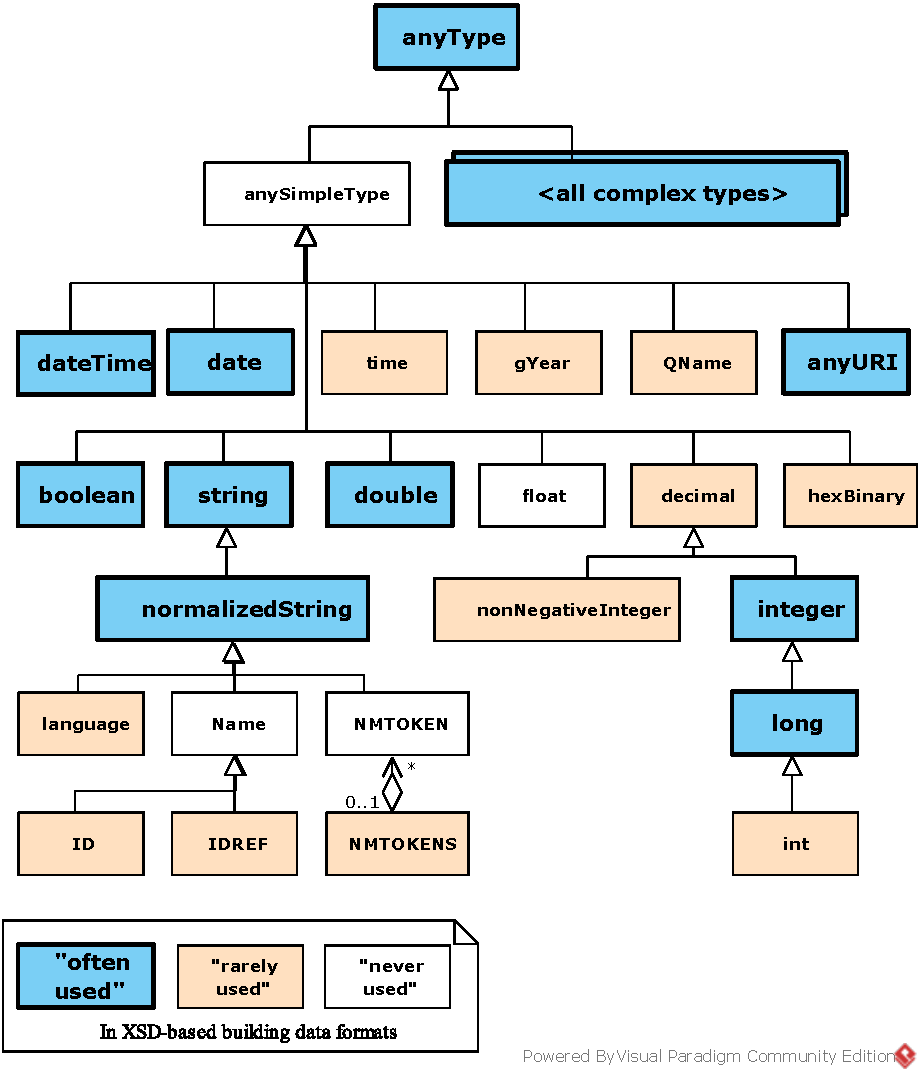
\includegraphics[width=\columnwidth]{images/xsd-type-hierarchy-8.pdf}
    % \caption{XSD type hierarchy\\\hspace{\textwidth}cyan, bold-border boxes}
     \caption{XSD types used in building data formats}
        % {\tabular[t]{@{}l@{}}XSD type hierarchy \\ This is the second line\endtabular}
    \label{fig:xsd-type-hierarchy}
\end{figure}




Simple type restriction \texttt{enumeration} is very often utilised in building data models for declaring enumeration types.
All 




